\section{Theory}

\subsection{Basis facts from electromagnetism}

This section is baed on chaptor 3 from the book \cite{wartak2013computational}


\subsubsection{Maxwell' equations}

Maxwell's equation describe the classic propagation of electromagnetic waves. These equations are given by

\begin{align}
\nabla \times \boldsymbol{E} &= - \frac{\partial \boldsymbol{B}}{\partial t} \\
\nabla \times \boldsymbol{H} &= \boldsymbol{J} + \frac{\partial \boldsymbol{D}}{\partial t} \\
\nabla \cdot \boldsymbol{D} &= \rho_v \\
\nabla \cdot \boldsymbol{B} &= 0~, 
\end{align}

where $\boldsymbol{E} / \boldsymbol{B}$ are the electric/magnetic field intensity, $\boldsymbol{B} / \boldsymbol{H}$ are the electric/magnetic flux density, $\boldsymbol{J}$ is the electric current density and $\rho_v$ is the volume charge density. Furthermore the following relations complement the relations between the vectorfields

\begin{align}
\boldsymbol{D} &= \epsilon \boldsymbol{E} \\
\boldsymbol{B} &= \mu \boldsymbol{H} \\
\boldsymbol{J} &= \sigma \boldsymbol{E}~,
\end{align}

where $\epsilon = \epsilon_0 \epsilon_r$ is the dielectric permittivity,  $\mu = \mu_0 \mu_r$ is the permeability and $\sigma$ is the electric conductivity.

The Maxwell's equatios can also be represented by an integral formulation. In this formualtions Gauss's and Stokes's theorem can be applied. By analyzing how the integral formulation of the Maxwell's equations behave at the boundary between two materials, one obtains the boundary conditions described in table \ref{tab:BCMaxwell}. A detailed derivation of the formulas can be found in \cite{wartak2013computational} chapter 3.2.

\begin{table}[h!]
\centering
\begin{tabular}{|c | c | c|} 
 \hline
 Field components & General form & Specific form  \\ [0.5ex] 
 \hline
 Tangential E & $\boldsymbol{n}_2 \times (\boldsymbol{E}_1 - \boldsymbol{E}_2) = 0 $ & $E_{1t} = E_{2t}$ \\ 
 Normal D & $\boldsymbol{n}_2 \cdot (\boldsymbol{D}_1 - \boldsymbol{D}_2) = \rho_s $ & $D_{1n} - D_{2n} = \rho_s$ \\
 Tangential H & $\boldsymbol{n}_2 \times (\boldsymbol{H}_1 - \boldsymbol{H}_2) = \boldsymbol{J}_s $ & $H_{1t} - H_{2t} = J_s$ \\
 Normal B & $\boldsymbol{n}_2 \cdot (\boldsymbol{B}_1 - \boldsymbol{B}_2) = 0 $ & $B_{1n} = B_{2n}$  \\ [1ex] 
 \hline
\end{tabular}
\caption{Table to test captions and labels.}
\label{tab:BCMaxwell}
\end{table}

We can see from table \ref{tab:BCMaxwell} that the tangential component of $E$ and the normal component of $B$ change continuously, whereas the normal component of $D$ and the tangential component of $H$ do not chamge continuously. An image describing the situation at the boundary can be seen in figure \ref{fig:BCMaxwell}.

\begin{figure}[h!]
    \centering
    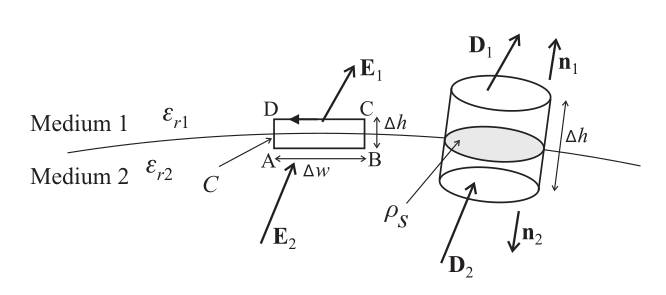
\includegraphics[width=0.8\textwidth]{figures/BCMaxwell.png}
    \caption{An interface between two media. Contour and volume used to derive boundary conditions for fields between two different dielectrics are shown. Image taken from \cite{wartak2013computational}.}
    \label{fig:BCMaxwell}
\end{figure}

\subsubsection{Wave equation}

A wave equation can be derived from a source free medium where $\rho_V = 0 = \boldsymbol{J}$ by applying $\nabla \times$ on both sides of the equation. The result is the follwoing wave equation

\begin{align}
\nabla^2 \boldsymbol{E} = \frac{n^2 \partial^2}{c^2\partial t^2} \boldsymbol{E}~,
\label{eq:waveequation}
\end{align}

where $c = \frac{1}{\sqrt{\mu_0 \epsilon_0}}$ is the speed of light and $n$ is the refractive index of the medium. In many practical situations the solution to the wave equation are time-harmonics, i.e. the solution can be written as 


\begin{align}
\boldsymbol{E} (\boldsymbol{r}, t) = \text{Re}\{ \boldsymbol{E}(\boldsymbol{r}) e^{i\omega t} \} ~,
\end{align}

where $\omega$ is the angular frequency. Often the fields can also be written as plane waves, i.e. in the form

\begin{align}
\boldsymbol{E} \propto e^{i\omega t - \boldsymbol{r} \boldsymbol{k}}~,
\end{align}

where $\boldsymbol{k}$ is the wave vektor. If both electric and magnetic fields can be written in this form, then the following relation between them holds

\begin{align}
\boldsymbol{k}\times \boldsymbol{E} = \omega \mu_0 \boldsymbol{H}.
\end{align}

This relation is visualized in figure \ref{fig:EMWaves}.

\begin{figure}[h!]
    \centering
    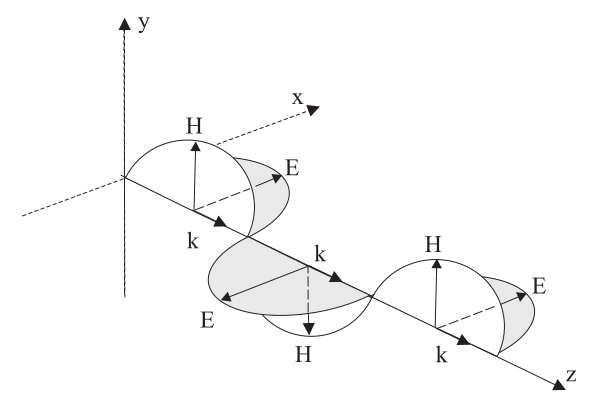
\includegraphics[width=0.6\textwidth]{figures/EMWaves.png}
    \caption{Visualization of the electric and magnetic fields from \cite{wartak2013computational}}
    \label{fig:EMWaves}
\end{figure}


\subsubsection{Polarized waves}

Polarization characterizes the curve which the $E$ vector makes (in the plane orthogonal to the direction of propagation) at a given point in space as a function of time. In the most general case, the curve produced is an ellipse and, accordingly, the wave is called elliptically polarized. Under certain conditions, the ellipse may be reduced to a circle or a segment of a straight line. In those cases it is said that the wave’s polarization is circular or linear, respectively. Since the magnetic field vector is related to the electric field vector, it does not need separate discussion. The different types of polarization can be seen in figure \ref{fig:Polarization}.

\begin{figure}[h!]
    \centering
    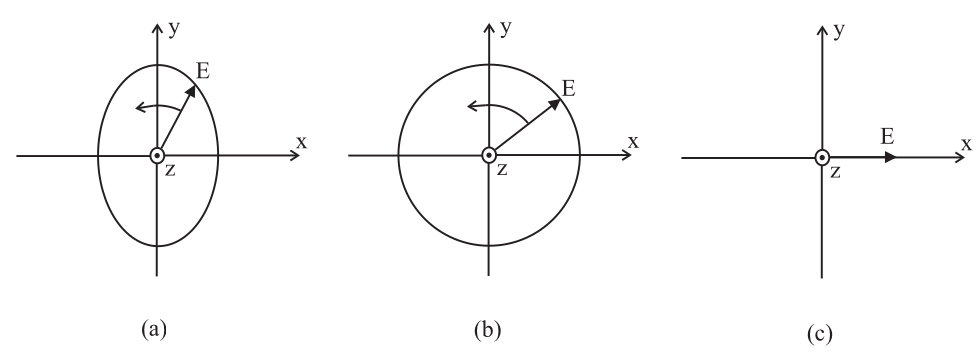
\includegraphics[width=0.8\textwidth]{figures/Polarization.png}
    \caption{Typical states of polarization: (a) elliptic, (b) circular and (c) linear from \cite{wartak2013computational}}
    \label{fig:Polarization}
\end{figure}

Furthermore, we distinguish between TE (or s) polarization and TM (or p) polarization. If a wave is TE polarized, then the electric field is normal to the plane of incidence (\textbf{s}enkrecht in german) or equivalent it is parallel to the the interface between both media. This configuration can  be seen in figure \ref{fig:TMPolarization}.

\begin{figure}[h!]
    \centering
    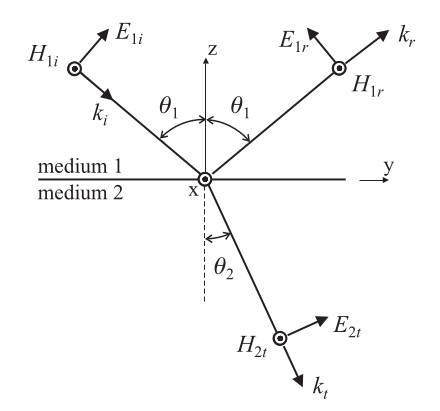
\includegraphics[width=0.4\textwidth]{figures/TMPolarization.png}
    \caption{Directions of vectors for a TM polarized wave from \cite{wartak2013computational}}
    \label{fig:TMPolarization}
\end{figure}

On the other hand, if a wave is TM polariced, then the electric field is \textbf{p}arallel to the to the plane of incidence. That implies that the magnetic field is normal to the plance of incidence.

\subsubsection{Snell's Law}

Snell's law describes how light behaves bewtween two isotropic materials. The setup can be seen in figure \ref{fig:snellsLaw}.

\begin{figure}[h!]
    \centering
    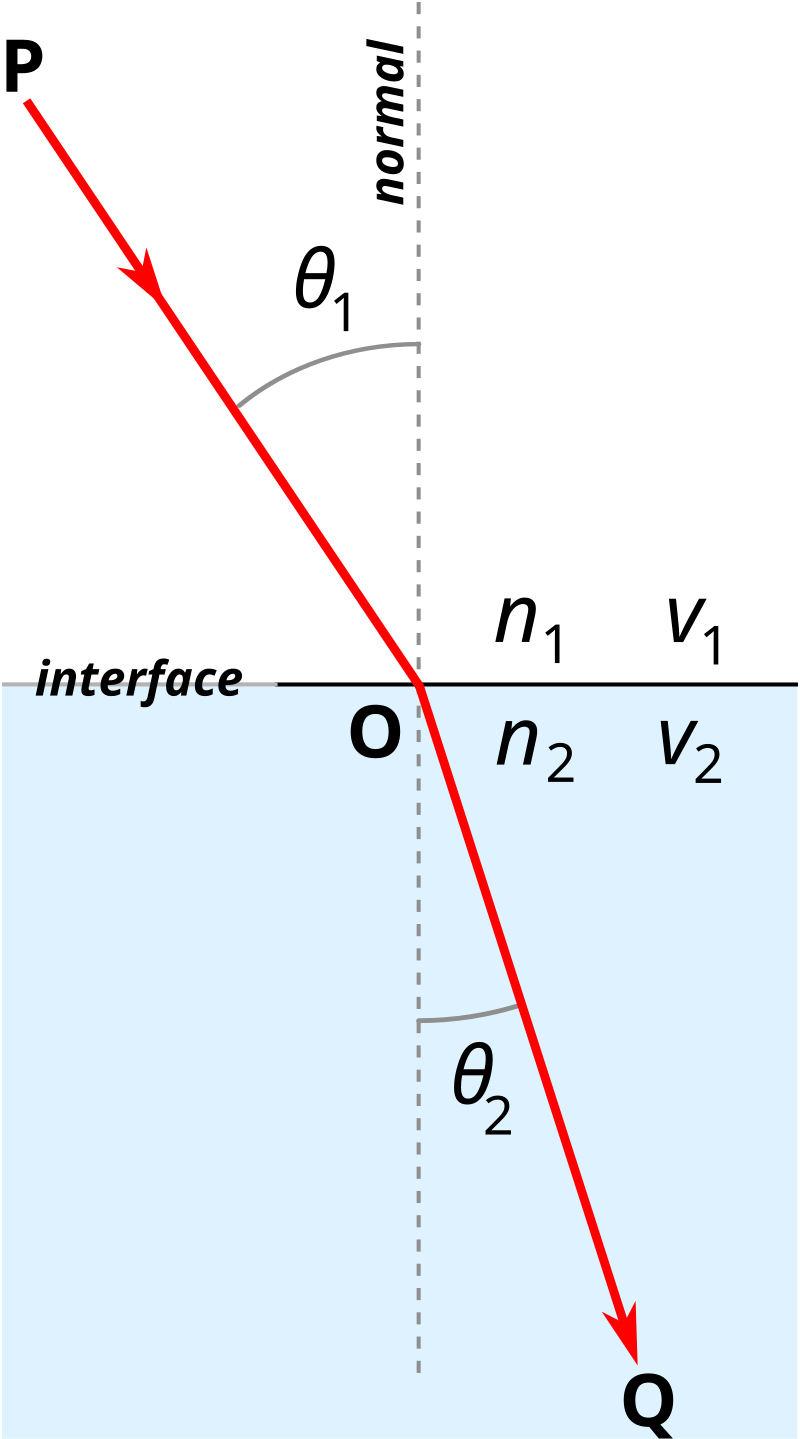
\includegraphics[width=0.2\textwidth]{figures/SnellsLaw2.png}
    \caption{Refraction of light at the interface between two media of different refractive indices, with $n_2 > n_1$. Since the velocity is lower in the second medium ($v_2 < v_1$), the angle of refraction $\theta_2$ is less than the angle of incidence $\theta_1$.}
    \label{fig:snellsLaw}
\end{figure}

Snell's law is described by the equation 

\begin{align}
\frac{\sin \theta_1}{\sin \theta_2} = \frac{n_2}{n_1} = \frac{v_1}{v_2}~,
\label{eq:SnellsLaw}
\end{align}

where $\theta_1$ is the angle of incident, $\theta_2$ is the angle of refraction, $n_{1/2}$ are the refrection indices associated to the isotropic materials and $v_{1/2}$ are the phase velocities in the two media. Snell's Law in \ref{eq:SnellsLaw} can be derived from \textit{Fermat's principle of least time}, which can be derived from the propagation of light waves. Fermat's theorem states that a path taken by a light ray between two given points is the one which minimizes the time.

\subsubsection{Fresnel coefficients and phases}

TODO


\subsubsection{Bragg Equation}


TODO
